\section{Die Schnelle Fourier-Transformation (FFT)}

Wir kommen nun zum Heiligen Gral in der Bildverarbeitung, nämlich der sogenannten \emph{Schnellen 
Fourier-Transformation (FFT)}. Da es sich dabei im um eine schnelle Implementierung der Diskreten 
Fourier-Transformation (DFT) handelt, wollen wir uns diese zunächst etwas genauer ansehen.

\subsection{Die Diskrete Fourier-Transformation (DFT)}

Wir werden nun kurz die Formel der Diskreten Fourier-Transformation herleiten. Die 
(kontinuierliche) Fourier-Transformation einer Folge $ c \in l_{1}(\Z) $ ist eine
$ 2\pi $-periodische Funktion $ \widehat{c} \in L_{1}(\T) $. Die einfachste Möglichkeit
$ \widehat{c} $ zu diskretisieren, ist $ \widehat{c} $ einfach an allen $ 2\pi / n $-ten Stellen 
für ein vorher gewähltes $ n \in \N $ abzutasten. So erhalten wir
\[
    \DFT_{n}
  \coloneq \widehat{c}_{n}
  \coloneq S_{2\pi / n} \ \widehat{c}
  = S_{2\pi / n} \ \sum_{k \in \Z} c(k) e^{-ik\bullet}
  = \sum_{k \in \Z} c(k) \ S_{2\pi / n} \ e^{-ik\bullet}
  = \sum_{k \in \Z} c(k) e^{-2\pi ik\bullet / n}.
\]

\begin{definition}[Diskrete Fourier-Transformation]
Zu einer Folge $ c \in l_{1}(\Z) $ bezeichnet man
\[
  \widehat{c}_{n} \coloneq \sum_{k \in \Z} c(k) e^{-2\pi ik\bullet / n}, \qquad n \in \N
\]
als die \emph{Diskrete Fourier-Transformation} (DFT) der Ordnung $ n $ von $ c $.
\end{definition}

\begin{remark}\leavevmode
\begin{itemize}
\item Die DFT $ \widehat{c}_{n} $ ist wegen
  \begin{align*}
      \widehat{c}_{n}(\bullet + n)
   &= \sum_{k \in \Z} c(k) e^{-2\pi ik(\bullet + n) / n}
    = \sum_{k \in \Z} c(k) e^{-2\pi ik(\bullet / n + 1)}
    = \sum_{k \in \Z} c(k) e^{-2\pi ik\bullet / n} \underbrace{e^{-2\pi ik}}_{=1} \\
   &= \sum_{k \in \Z} c(k) e^{-2\pi ik\bullet / n} = \widehat{c}_{n}(\bullet)
  \end{align*}
  $ n $-periodisch. Das heißt, sie ist durch die Werte
  \[
    \widehat{c}_{n}(k), \qquad k \in \Z_{n} = \Z / n\Z \simeq \{0, 1, \ldots, n - 1\}
  \]
  eindeutig festgelegt.
\item Für $ m $-periodische oder $ m $-periodisierte Folgen $ c \in l(\Z_{m}) $ lässt sich die DFT 
  der Ordnung $ n $ auch als Matrix darstellen:
  \[
    \widehat{c}_{n} = V_{n,m}c, \qquad
    V_{n,m} \coloneq \left( e^{-2\pi i j k / n} : j \in \Z_{n}, k \in \Z_{m} \right) 
      \in \C^{n \times m}.
  \]
  Die Matrix $ V_{n,m} $ bezeichnen wir auch als \emph{Transformationsmatrix}.
\item Ist $ m = n $, so schreiben wir statt $ V_{n,n} $ einfach $ V_{n} $. In diesem Fall definieren
  wir die primitive $ n $-te Einheitswurzel
  \[
    \omega \coloneq e^{-2\pi i / n}, \qquad \omega^{n} = e^{-2\pi i} = 1.
  \]
  Dann gilt
  \[
      V_{n} 
    = \left( \omega^{jk} : j,k \in \Z_{n} \right)
    = \begin{pmatrix}
        1 		 & 1 						 	& 1 				 & \cdots & 1 & 1 \\
        1 		 & \omega				  & \omega^{2} & \cdots & \omega^{n - 2} & \omega^{n - 1} \\
        1 		 & \omega^{2} 		& \omega^{4} & \cdots & \omega^{2(n - 2)} & \omega^{2(n - 1)} \\
        \vdots & \vdots 				& \vdots & \ddots 	& \vdots & \vdots \\
        1 		 & \omega^{n - 2} & \omega^{2(n - 2)} & \cdots & \omega^{4} & \omega^{2} \\
        1 		 & \omega^{n - 1} & \omega^{2(n - 1)} 		& \cdots & \omega^{2} & \omega
      \end{pmatrix}.
  \]
  Das heißt, die Matrix ist symmetrisch und besitzt vollen Rang, weshalb sie insbesondere immer 
  invertierbar ist. Sie definiert einen Basiswechsel vom Ort-/Zeitbereich in den Frequenzbereich.
\end{itemize}
\end{remark}

\begin{proposition}[Inverse DFT]
Für ein $ n \in \N $ ist die Inverse DFT zu $ V_{n} $ gegeben durch
\[
    V_{n}^{-1}
  = \frac{1}{n} \left( e^{2\pi i j k / n} : j \in \Z_{n}, k \in Z_{m} \right)
  = \frac{1}{n} \left( \omega^{-jk} : j,k \in \Z_{n} \right).
\]
\end{proposition}

\begin{example}[Berechnung der Transformationsmatrix]
Für $ n = 4 $ ist
\[
    V_{4}
  = \begin{pmatrix*}[r]
      1 &  1 &  1 &  1 \\
      1 &  i & -1 & -i \\
      1 & -1 &  1 & -1 \\
      1 & -i & -1 & i
    \end{pmatrix*}, \qquad
    V_{4}^{-1}
  = \frac{1}{4} \begin{pmatrix*}[r]
      1 &  1 &  1 &  1 \\
      1 & -i &  1 &  i \\
      1 &  1 & -1 &  1 \\
      1 &  i &  1 & -i
    \end{pmatrix*},
\]
das heißt
\[
    V_{4} \ V_{4}^{-1}
  = \frac{1}{4} \begin{pmatrix}
      4 & 0 & 0 & 0 \\
      0 & 4 & 0 & 0 \\
      0 & 0 & 4 & 0 \\
      0 & 0 & 0 & 4
    \end{pmatrix}
  = \begin{pmatrix}
      1 & 0 & 0 & 0 \\
      0 & 1 & 0 & 0 \\
      0 & 0 & 1 & 0 \\
      0 & 0 & 0 & 1
      \end{pmatrix}.
\]
\end{example}

\begin{example}[Die DFT in Aktion]
Tasten wir einmal den Cosinus an $ 512 $ äquidistanten Punkten im Intervall $ [0, 2\pi) $ ab,
d.h.\ wir berechnen $ S_{2\pi/512}\cos $, und bestimmen wir zu dieser Diskretisierung die DFT der 
Ordnung $ 512 $. Vorüberlegungen:
\begin{itemize}
\item Der Cosinus ist eine gerade Funktion. D.h.\ die DFT des Cosinus ist vollständig
  reellwertig.
\item Der Cosinus lässt sich auch schreiben als
  \[
      \cos(x) 
    = \frac{e^{ix} + e^{-ix}}{2}
    = \frac{e^{\mathbf{1} \cdot ix}}{2} + \frac{e^{\mathbf{-1} \cdot ix}}{2},
  \]
  d.h.\ es treten nur die beiden Frequenzen $ 1 $ und $ -1 \simeq 511 $ im Signal auf, welche beide 
  den gleichen relativen Anteil am Signal haben. Da wir eine DFT der Ordnung $ 512 $ verwenden, 
  können wir $ 512 $ verschiedene Frequenzen unterscheiden. Der absolute Anteil der beiden
  oben erwähnten Frequenzen sollte also jeweils $ 512 / 2 = 256 $ sein. Oder anders gesagt:
  Im Funktionsplot der DFT muss es an den Stellen $ \frac{2\pi}{512} $ und
  $ \frac{2\pi}{512} \cdot 511 $ einen Ausschlag von jeweils $ 256 $ geben. Und genau das ist auch 
  der Fall, wie Abbildung~\ref{fig:dft512_cosine} zeigt. Alle anderen Frequenzen haben keinen 
  Anteil am Signal, was auch in der Abbildung zu sehen ist.
  \begin{figure}
  \centering
  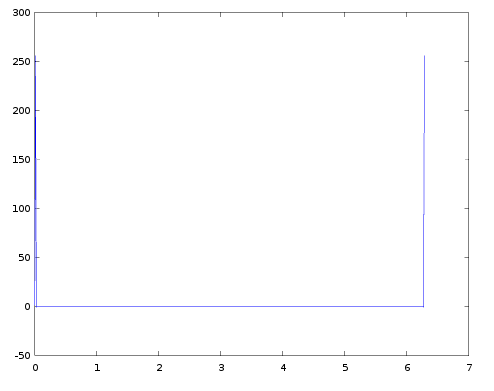
\includegraphics[width=0.5\linewidth]{Bilder/dft512_cosine}
  \caption{DFT der Ordnung $ 512 $ zu $ S_{2\pi/512}\cos $.}
  \label{fig:dft512_cosine}
  \end{figure}
\end{itemize}
\end{example}

Wir wollen nun ein paar wichtige Eigenschaften der Diskreten Fourier-Transformation in Anlehnung
an Bemerkung~\ref{prop:properties_fourier} zusammenstellen. Dazu definieren wir uns noch schnell den
Begriff der Zyklischen Faltung.

\begin{definition}[Zyklische Faltung]
Zu zwei periodischen Folgen $ c, d \in l(\Z_{n}) $ ist die \emph{zyklische Faltung}
$ c * d = c *_{n} d \in l(\Z_{n}) $ definiert als
\[
  (c *_{n} d)(j) = \sum_{k \in \Z_{n}} c(k) d(j - k), \qquad j \in \Z_{n}.
\]
Dabei ist der Ausdruck $ j - k $ den Rechenregeln in $ \Z_{n} $, also modulo $ n $, zu verstehen.
\end{definition}

\begin{proposition}[Eigenschaften der DFT]
Für $ n \in \N $ und $ c, d \in l(\Z_{n}) $ gilt:
\begin{enumerate}
\item $ \DFT_{n} \colon l(\Z_{n}) \rightarrow l(\Z_{n}) $ ist eine invertierbare lineare Abbildung
  mit
  \[
    \norm{c}_{2} = \frac{1}{\sqrt{n}} \norm{\widehat{c}_{n}}_{2}.
  \]
  Dabei sind die $ p $-Normen definiert als
  \[
    \norm{c}_{p} \coloneqq \left( \sum_{k \in \Z_{n}} |c(k)|^{p} \right)^{1/p}
  \]
  bzw.
  \[
    \norm{c}_{\infty} \coloneqq \max_{k \in \Z_{n}} |c(k)|.
  \]
\item Es gilt
  \[
    (c *_{n} d)_{n}^{\wedge} = \widehat{c_{n}} \odot \widehat{d_{n}}.
  \]
  Die Multiplikation $ \odot $ auf der rechten Seite ist dabei als punktweises Produkt von Vektoren 
  zu verstehen: 
  $ \left( \widehat{c_{n}} \odot \widehat{d_{n}} \right)(j) = 
    \widehat{c_{n}}(j) \cdot \widehat{d_{n}}(j) $ (sog.\ \emph{Hadamard-Produkt}).
\end{enumerate}
\end{proposition}

\begin{remark}[DFT im Zweidimensionalen]
Für zweidimensionale Signale $ c \in l(\Z_{n}^{2}) $ (also bspw.\ gekachelte Bilder) gilt
\begin{align*}
     \widehat{c}(\beta)
  &= \sum_{\alpha \in \Z_{n}^{2}} c(\alpha) e^{-2\pi i \alpha^{\top} \beta / n}
   = \sum_{\alpha_{1} \in \Z_{n}} \sum_{\alpha_{2} \in \Z_{n}}
       c(\alpha_{1}, \alpha_{2}) e^{-2 \pi i \alpha_{1} \beta_{1} / n} 
       e^{-2 \pi i \alpha_{2} \beta_{2} / n} \\
  &= \sum_{\alpha_{1} \in \Z_{n}} e^{-2 \pi i \alpha_{1} \beta_{1} / n}
        \underbrace{\sum_{\alpha_{2} \in \Z_{n}} c(\alpha_{1}, \alpha_{2}) 
          e^{-2 \pi i \alpha_{2} \beta_{2} / n}}_{
            = (c(\alpha_{1}, \bullet))^{\wedge}(\beta_{2})} \\
  &= \sum_{\alpha_{1} \in \Z_{n}} (c(\alpha_{1}, \bullet))^{\wedge}(\beta_{2})
        e^{-2 \pi i \alpha_{1} \beta_{1} / n}.
\end{align*}
Diese Formel liefert uns eine Berechnungsmethode für zweidimensionale DFTs:
\begin{enumerate}
\item Zuerst bildet man die eindimensionale DFT für jede Zeile der Matrix $ c $. Dies liefert uns
  einen Ergebnisvektor mit den Einträgen $ (c(0, \bullet))^{\wedge} $ bis
  $ (c(n - 1, \bullet))^{\wedge} $.
\item Diesen Ergebnisvektor müssen wir nun nochmals mit der eindimensionalen DFT transformieren.
  Das Ergebnis dieses Vorgangs ist dann die Fourier-Transformation $ \widehat{c} $ unserer Matrix.
\end{enumerate}
Schematische Darstellung:
\[
  \begin{array}{ccccc}
    c(0,0) & \cdots & c(0, n -1) & \rightarrow & (c(0, \bullet))^{\wedge} \\
    c(1,0) & \cdots & c(1, n -1) & \rightarrow & (c(1, \bullet))^{\wedge} \\
    \vdots & \ddots & \vdots	   &   					 & \vdots \\
    c(n - 1, 0) & \cdots & c(n - 1, n -1) & \rightarrow & (c(n - 1, \bullet))^{\wedge} \\
    & & & & \downarrow \\
    & & & & \widehat{c}
  \end{array}
\]
Das heißt, wir benötigen insgesamt $ n + 1 $ eindimensionale DFTs, und deswegen hängt die
Performance der zweidimensionalen DFT signifikant von der eindimensionalen DFT ab.
\end{remark}

\subsection{Diskret vs.\ Diskretisiert}
Dieser Teil thematisiert die Probleme, die auftreten, wenn man versucht, aus der DFT
eines abgetasteten kontinuierlichen Signals $ f $ die Fourier-Transformation von $ f $ zu 
rekonstruieren. Als Beispiel wurde im Skript die DFT der $ \sinc $-Funktion angeführt. Diese führt
nämlich nicht zur Rechtecksfunktion, wie man eigentlich erwarten würde, sondern zu zwei
\enquote{Teufelshörnern}. Um die Bildung von solchen Artefakten beim Rekonstruktionsvorgang zu 
vermeiden, kann man versuchen, $ f $ mittels eines sog.\ \emph{Quasi-Interpolanten} zu 
approximieren. Häufig verwendete Quasi-Interpolanten sind die kardinalen Splines. Interessant sind 
eigentlich nur diese beiden Punkte:
\begin{enumerate}
\item Die Schrittweite $ h $ der Abtastung von $ f $ bestimmt, welche Frequenzen von $ f $ wirklich
  in der DFT der Abtastung von $ f $ codiert sind. Je feiner die Abtastung, desto mehr Frequenzen 
  werden codiert.
\item Die Frequenzauflösung, also die Zahl der Frequenzen, die sich in der DFT unterscheiden lassen,
  hängt hingegen von der Ordnung $ n $ der DFT ab. Je größer $ n $ gewählt wird, umso feiner die
  Frequenzauflösung. Und je kleiner $ n $, umso mehr nicht zusammengehörige Frequenzen werden zu
  einer Frequenz zusammengefasst.
\end{enumerate}
Aber das hätte man sich auch so irgendwie denken können\dots

\subsection{Die Schnelle Fourier-Transformation}

Wie wir jetzt wissen, lässt sich die Diskrete Fourier-Transformation naiv als 
Matrix-Vektor-Multiplikation implementieren. Dies ist aber nicht sonderlich effizient, da im Falle
einer DFT der Ordnung $ n $ somit $ \mathcal{O}(n^{2}) $ Rechenoperationen (sprich Multiplikationen
und Additionen) durchzuführen sind. Aufgrund der enormen Bedeutung der DFT in den modernen
Wissenschaften und deren weit verbreitetem Einsatz in laufzeitkritischen Anwendungen hätte man 
gerne eine effizientere Möglichkeit, die DFT zu berechnen. Und genau das leistet die \emph{Schnelle 
Fourier-Transformation} (FFT). Sie verringert die Kosten der Berechnung auf
$ \mathcal{O}(n \log(n)) $.

Es gibt eigentlich gar nicht \enquote{die eine} FFT, sondern mehrere Varianten der FFT, welche alle 
abhängig von der Dimension oder der Struktur des Eingabevektors ihre Vor- und Nachteile haben. Die 
allgemeinste und geläufigste Variante der FFT ist das Verfahren nach James Cooley und John Tukey. 
Dieses wollen wir im Folgenden studieren.

Hinter der Cooley-Tukey-FFT steckt ein einfacher Divide-and-Conquer-Algorithmus. Angenommen, unser
zu transformierendes Signal der Länge $ n $ ist $ c \in l(\Z_{n}) $, wobei $ n = 2m $ eine gerade 
Zahl ist. Dann können wir die Fourier-Transformation von $ c $ für ein $ j \in \Z_{n} $ auch
schreiben als
\[
    \widehat{c_{n}}(j) 
  = (c(2\bullet))_{m}^{\wedge}(j) + \omega^{j} \ (c(2\bullet + 1))_{m}^{\wedge}(j).
\]
Das bedeutet: Wir halbieren den Eingabevektor der Länge $ n $ in zwei kleinere Vektoren der Länge
$ m $, indem wir jeweils nur gerade bzw.\ ungerade Indizes betrachten. Danach berechnen wir für 
diese zwei Vektoren jeweils die DFT der Ordnung $ m $. Die resultierenden Ergebnisvektoren setzen 
wir anschließend wieder geschickt zusammen, um so das eigentliche Ergebnis der DFT von $ c $ zu 
erhalten.

Wenden wir dieses Verfahren rekursiv so lange an, bis wir irgendwann nur noch (Teil-)Vektoren der 
Länge $ 2 $ zu verarbeiten haben (deren DFT wir direkt berechnen können), ergibt sich nach dem
Master-Theorem eine Komplexität von $ \mathcal{O}(n \log(n)) $. Dies ist typisch für solche 
Baumalgorithmen. Denn die Tiefe des Berechnungsbaumes ist ja gerade in $ \mathcal{O}(\log n) $ und
die Anzahl der Blätter ist in $ \mathcal{O}(n) $. Da wir aus den Blättern des Baumes die 
Gesamtlösung
zusammensetzen müssen, ergibt sich somit die oben erwähnte Gesamtkomplexität von
$ \mathcal{O}(n \log(n)) $.

Die Form der Cooley-Tukey-FFT, die wir gerade betrachtet haben, ist die sog.\ \emph{Radix-$ 2 
$-FFT}, da wir die Eingabevektoren immer in zwei Teile zerlegt haben. Darüber hinaus gibt es die 
Möglichkeit, die Vektoren jeweils in $ p $ Teile zu zerlegen, für den Fall, dass $ n $ keine gerade 
Zahl sein sollte. Dies führt dann zu der allgemeinen \emph{Radix-$ p $-FFT}. Hier sind also mehr 
DFTs für kürzere Segmente zu berechnen, was aber in der $ \mathcal{O} $-Notation immer noch eine 
Laufzeitkomplexität von $ \mathcal{O}(n\log(n)) $ ergibt.

Wie würde die Cooley-Tukey-FFT zu einer $ \DFT_{4} $ aussehen? Nun, wenn wir die DFT wieder als
Matrix-Vektor-Multiplikation auffassen, dann stellt sich heraus, dass sich die Transformationsmatrix
$ V_{4} $ mit der oben beschriebenen Berechnungsvorschrift in vier dünn besetzte Matrizen 
faktorisieren lässt:
\[
\begin{pmatrix*}[r]
      1 &  1 &  1 &  1 \\
      1 &  i & -1 & -i \\
      1 & -1 &  1 & -1 \\
      1 & -i & -1 & i
    \end{pmatrix*}
=
\underbrace{
\begin{pmatrix*}[r]
1 & \cdot & 1 & \cdot \\ \cdot & 1 & \cdot & 1 \\ 1 & \cdot & -1 & \cdot \\ \cdot & 1 & \cdot & -1
\end{pmatrix*}
}_{= \DFT_{2} \otimes I_{2} \coloneqq M_{4}}
\underbrace{
\begin{pmatrix}
1 & \cdot & \cdot & \cdot \\ \cdot & 1 & \cdot & \cdot \\ \cdot & \cdot & 1 & \cdot \\ \cdot & 
\cdot & \cdot & i
\end{pmatrix}
}_{\coloneqq M_{3}}
\underbrace{
\begin{pmatrix*}[r]
1 & 1 & \cdot & \cdot \\ 1 & -1 & \cdot & \cdot \\ \cdot & \cdot & 1 & 1 \\ \cdot & \cdot & 1 & -1
\end{pmatrix*}
}_{= I_{2} \otimes \DFT_{2} \coloneqq M_{2}}
\underbrace{
\begin{pmatrix}
1 & \cdot & \cdot & \cdot \\ \cdot & \cdot & 1 & \cdot \\ \cdot & 1 & \cdot & \cdot \\ \cdot & 
\cdot & \cdot & 1
\end{pmatrix}.
}_{\coloneqq M_{1}}
\]
Und damit gilt für ein Eingabesignal $ x \in l(\Z_{4}) $
\[
  \begin{pmatrix}
  y_{1} \\ y_{2} \\ y_{3} \\ y_{4}
  \end{pmatrix}
  =
  V_{4}   \begin{pmatrix}
    x_{1} \\ x_{2} \\ x_{3} \\ x_{4}
  \end{pmatrix}
  = 
  M_{4} M_{3} M_{2} M_{1}   \begin{pmatrix}
      x_{1} \\ x_{2} \\ x_{3} \\ x_{4}
    \end{pmatrix}.
\]
Diese Berechnung ist in Abbildung~\ref{fig:cooley-tukey-fft} schematisch dargestellt.
\begin{figure}[ht]
\centering
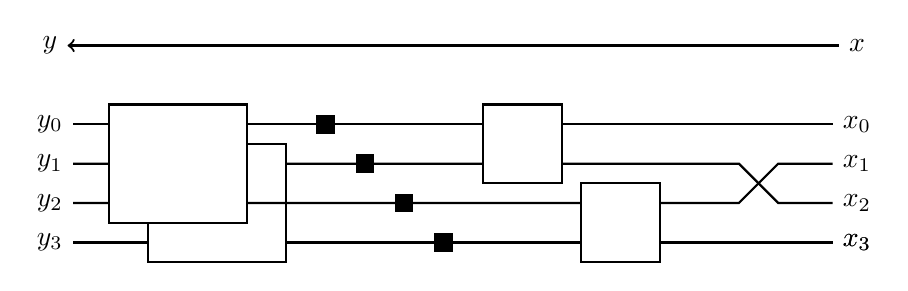
\begin{tikzpicture}[thick]

  \node (y) at (0, 2.5) {$ y $};
  \node (x) at (10.25, 2.5) {$ x $};
  \draw [->] (x) -- (y);

  \node (y0) at (0,1.5) {$ y_{0} $};
  \node (y1) at (0,1) {$ y_{1} $};
  \node (y2) at (0,0.5) {$ y_{2} $};
  \node (y3) at (0,0) {$ y_{3} $};
  
  \node (x0) at (10.25,1.5) {$ x_{0} $};
  \node (x1) at (10.25,1) {$ x_{1} $};
  \node (x2) at (10.25,0.5) {$ x_{2} $};
  \node (x3) at (10.25,0) {$ x_{3} $};
  
  \draw (y3) -- (x3);
  \draw (y0) -- (x0);
  
  \draw (y1) -- (8.75, 1) -- (9.25,0.5) -- (x2);
  
  \filldraw[draw=black, fill=white] (1.25,1.25) rectangle (3,-0.25);
  
  \draw (y2) -- (8.75, 0.5) -- (9.25,1) -- (x1);
  
  \filldraw[draw=black, fill=white] (0.75,1.75) rectangle (2.5,0.25);
  
  \node [rectangle,fill=black] at (3.5,1.5) {};
  \node [rectangle,fill=black] at (4,1) {};
  \node [rectangle,fill=black] at (4.5,0.5) {};
  \node [rectangle,fill=black] at (5,0) {};
  
  \filldraw[draw=black, fill=white] (5.5, 1.75) rectangle (6.5, 0.75);
  \filldraw[draw=black, fill=white] (6.75, 0.75) rectangle (7.75, -0.25);
  
  \node (x3) at (10.25,0) {$ x_{3} $};
  
%  \draw [dashed] (0.5,2) rectangle (5.2,-0.5);
%  \draw [dashed] (5.4,2) rectangle (9.5,-0.5);
  
  \end{tikzpicture}
  \caption{Datenflussdiagramm zur Cooley-Tukey-FFT der Ordnung $ 4 $. Man beachte, dass die Daten
  von rechts nach links fließen. Die weißen Kästchen symbolisieren eine DFT der Ordnung $ 2 $,
  die schwarzen Kästchen eine Skalierung der Daten durch $ \omega^{j} $.}
  \label{fig:cooley-tukey-fft}
\end{figure}
Zur Erklärung: Die Matrix $ M_{1} $ bewirkt die Aufteilung des Eingabevektors in gerade und ungerade
Indizes. Die Matrix $ M_{2} $ führt anschließend jeweils eine $ \DFT_{2} $ auf den Teilvektoren 
durch. Danach erfolgt eine Skalierung der Daten durch $ M_{3} $ (dies entspricht dem Korrekturterm
$ \omega^{j} $). Abhängig von der Wahl von $ j $ müssen die beiden Vektoren nun wieder zu einem
großen Vektor zusammengesetzt werden, was durch $ M_{4} $ geschieht. Unter der Annahme, dass 
Multiplikationen mit $ 1 $ und $ -1 $ sowie Additionen mit $ 0 $ wegoptimiert werden können, 
benötigt dieser ganze Vorgang insgesamt nur drei Additionen und vier Multiplikationen, wohingegen 
beim naiven Ansatz über die Transformationsmatrix $ V_{4} $ zwölf Additionen und vier 
Multiplikationen auszuführen sind.

Neben der Cooley-Tukey-FFT gibt es u.a.\ noch die
\begin{itemize}
\item \emph{Prime-factor FFT} (für den Fall, dass $ n = km $ und $ \gcd(k,m) = 1 $),
\item \emph{Rader FFT} (falls $ n $ eine Primzahl ist),
\item \emph{Bluestein FFT}.
\end{itemize}

\subsection{Fourier und Bilder}

Dank der FFT lassen sich digitale Filter schnell und effizient am Rechner implementieren. Dies kann
man sich z.B.\ bei der Bildkomprimierung zunutze machen. Die Idee dabei ist, dass man gewisse
hochfrequente Anteile eines Bildes (feine Texturen, Details usw.) zu einem gewissen Grad aus dem
Bild entfernen kann, ohne dass dies vom menschlichen wahrgenommen wird. So muss weniger Information
im Bild gespeichert werden.

Das gegebene Bild wird hierzu in gleichgroße Blöcke (z.B.\ der Größe $ 8 \times 8 $ zur 
Verarbeitung mit Grafikkarten) aufgeteilt, welche nun alle separat Fourier-transformiert werden.
Dieser Vorgang lässt sich hervorragend parallelisieren, da zwischen den Blöcken keinerlei 
Abhängigkeiten bestehen. Anschließend wird auf jeden dieser Blöcke ein Tiefpassfilter (bspw.\ eine 
diskretisierte Variante eines Binomalfilters) angewendet, um so nur noch die groben Informationen
des Bildes zu behalten. Auch dieser Vorgang lässt sich über die FFT ausgesprochen schnell 
durchführen. Abhängig von den Eigenschaften des verwendeten Tiefpassfilters und der gewählten 
Blockgröße wird das Bild nun mehr oder weniger stark komprimiert worden sein.

Um das resultierende Bild betrachten zu können, muss die Inverse Fourier-Transformation auf jedem 
der Blöcke ausgeführt werden, da die Bildinformationen ja im Frequenzbereich vorliegen und erst 
noch in der Ortsbereich überführt werden müssen. Je nach Kompressionsrate des Bildes kann verstärkt 
Artefaktbildung (Blöcke, Ringe usw.) aufgetreten sein, da das hier beschriebene Verfahren nicht 
verlustfrei arbeitet.

Dies ist auch die grobe Idee hinter dem Kompressionsverfahren, welches bei JPEG zum Einsatz kommt. 
Im Gegensatz zur Fourier-Transformation wird bei JPEG auf die \emph{Diskrete Cosinus-Transformation}
zurückgegriffen. Diese liefert nur reellwertige Ergebnisse und eignet sich daher wesentlich besser
für die Verarbeitung mit modernen Rechnern. Die bereits komprimierten Daten des Bildes können bei
JPEG z.B.\ durch das sog.\ \emph{Huffman-Encoding} nochmals komprimiert werden, und zwar 
verlustfrei.

\begin{definition}[Diskrete Cosinus-Transformation (DCT)]
Die DCT bildet einen Vektor $ f \in l(\Z_{n}) $ auf eine Linearkombination an Cosinus-Termen ab.
Diese Operation ist insbesondere invertierbar und linear. Von den vier Typen der DCT ist die 
gebräuchlichste Variante definiert durch
\[
  \DCT2 f(j) = \sum_{k \in \Z_{n}} f(k) \cos \left( \frac{\pi (k + \frac{1}{2})j}{n} \right).
\]
Auf Basis der FFT lässt sich auch die DCT effizient in $ \mathcal{O}(n \log(n)) $ berechnen.
\end{definition}